\section{Colored Petri Net-based Analysis Model}
\label{sec:Colored_Petri Net-based_Analysis_Model}

This section briefly describes how Colored Petri nets (CPN) are used to build an extensible, scalable analysis model for component-based applications. Several nets are used to compose the different layers of the design model. To edit, simulate and analyze this model, we use the CPN Tools \cite{CPNTools} tool suite. The tool suite includes a simulator, as well as a state-space analysis tool that computes the (bounded) state space of the system under execution. The analysis model is based on the formal component model, i.e. the model of computation used. For a different component execution semantics, this model needs to be adjusted. 

\subsection{Model of Time}
Appropriate choice for temporal resolution is a necessary first step in order to model and analyze threads running on a processor. The OS scheduler enforces temporal partitioning and uses a priority-based scheme for threads active within a temporal partition. If multiple threads have the same priority, a round-robin (RR) scheduling is used. In order to observe and analyze this behavior, we have chosen the temporal resolution to be 1 ms; a fraction of 1 clock tick of the OS scheduling quantum. 
\subsubsection{Dynamic Time Progression}
Although the time resolution at the start of the analysis is chosen to be 1 ms, this is not a constant throughout the execution of the analysis model. If it were then \emph{S} seconds of activity will generate a state space of size: $SS_{size} = \sum\limits_{i=1}^{S*1000} TF_{t_i}$
%\vspace{-0.2in}
%
%\begin{equation}
%\begin{split}
%SS_{size} = \sum\limits_{i=1}^{S*1000} & TF_{t_i}
%\end{split}
%\end{equation}
where $TF_{t_i}$ is the number of state-changing CPN transition firings between $t_i$ and $t_{i+1}$. This large state space includes intervals of time where there is no thread activity to analyze either due to lack of operation requests, lack of ready threads for scheduling, or due to temporal partitioning. During such idle periods, the analysis engine dynamically increases the time-step size and progresses time either to (1) the next node-specific clock tick, (2) the next global timer expiry offset, or (3) the next node-specific temporal partition (whichever is earliest and most relevant). This ensures that the generated state space tree is devoid of nodes where there is no thread activity. Such dynamic control of time using global variables during analysis is also one of the advantages of using colored Petri nets. 

\subsection{Modeling Component-based Applications}

\begin{figure}[htb]
	\centering
	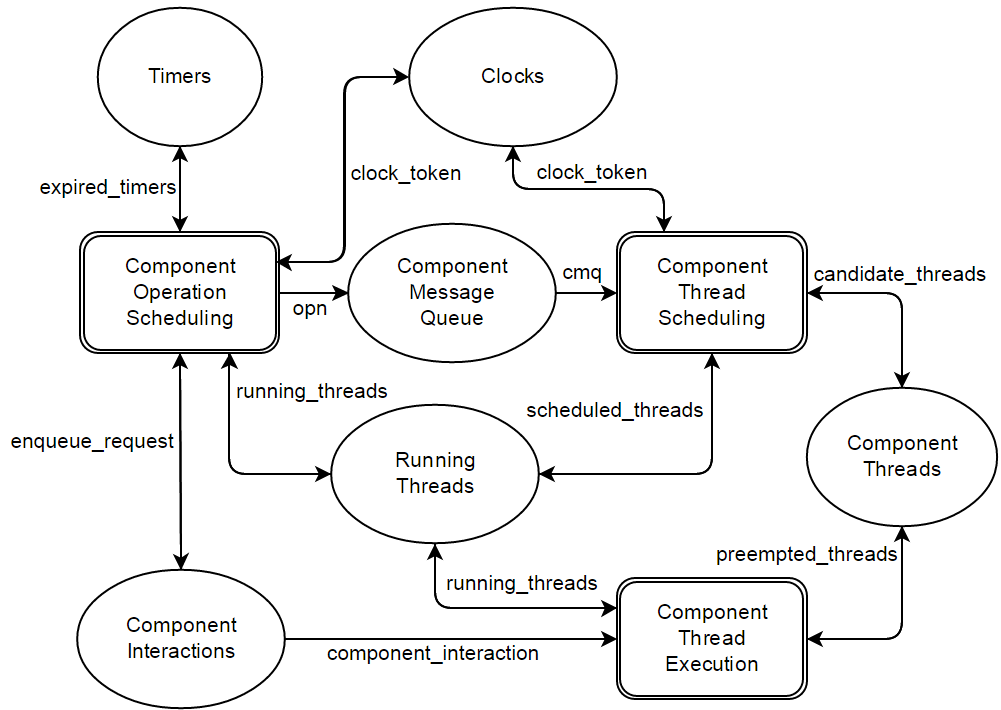
\includegraphics[width=0.45\textwidth]{figs/HL_CPN.png}
	\caption{Top-level CPN Model}
	\label{fig:hl_cpn}
\end{figure}

The top-level CPN Model is shown in Figure \ref{fig:hl_cpn}. The places (shown as ovals) in this model maintain \emph{colored} (typed) tokens that represent the states of interest for analysis. For instance, the \emph{Clocks} place holds tokens of type \emph{clock\_tokens} maintaining information regarding the state of the clock values and temporal partition schedule on all computing nodes. To ensure modularity, this model is partitioned into two interacting sub-nets to handle the hierarchical scheduling.

\subsubsection{Component-level Execution Model}

\paragraph{Component Operations} Every operation request \emph{O} made on a component \emph{$C_x$} is a \emph{record} type implementation of the 4-tuple:

\vspace{-0.15in}
\begin{equation}
O(C_x) = \ < ID_O, \ Prio_O, \ Dl_O, \  Steps_O >
\end{equation}

where, $ID_O$ is a unique concatenation of strings that help identify and locate this operation in the system (consisting of the name of the operation, the component, the computing node, and the temporal partition). The operation's priority ($Prio_O$) is used by the analysis engine to enqueue this operation request on the message queue of $C_x$ using a fixed-priority non-preemptive FIFO scheduling scheme. The completion of this enqueue implies that this operation has essentially been \emph{scheduled} for execution. Once enqueued, if this operation does not execute and complete before its fixed deadline ($Dl_O$), its real-time requirements are violated. 

\paragraph{Steps} 
\label{para:steps}

Once an operation request is dequeued, the execution of the operation is modeled as a transition system that runs through a sequence of steps dictating its behavior. Any of these underlying steps can have a state-changing effect on the thread executing this operation. For example, interactions with I/O devices on the component-level could block the executing thread (for a non-deterministic amount of time) on the OS-level. Therefore, every component operation has a unique list of steps ($Steps_O$) that represent the sequence of local or remote interactions undertaken by the operation. Each of the \emph{m} steps in $Steps_O$ is a 4-tuple:

\vspace{-0.15in}
\begin{equation}
s_i = \ <Port, \ Unblk_{s_i}, \ Dur_t, \ Exec_t>
\end{equation}

where $1 \le i \le m$. \emph{Port} is a \emph{record} representing the exact communication port used by the operation during $s_i$. $Unblk_{s_i}$ is a list of component threads that are unblocked when $s_i$ completes. This list is used, e.g., when the completion of a synchronous remote method invocation on the server side is expected to unblock the client thread that made the invocation. Finally, temporal behavior of $s_i$ is captured using the last two integer fields: \emph{$Dur_t$} is the worst-case estimate of the time taken for $s_i$ to complete and $Exec_t$ is the relative time of the execution of $s_i$, with $0 \le Exec_t \le Dur_t$.

\paragraph{Component Interactions}

Consider an application with two components: a client and a server. The client is periodically triggered by a timer to make an remote method call to the server. We know that when the client executes an instance of the timer-triggered operation, a related operation request is enqueued on the server's message queue. In reality, this is handled by the underlying middleware. Since we do not model the details of this framework, the server-side request is modeled as an \emph{induced operation} that manifests as a consequence of the client-side activity. Tokens that represent such design-specific interactions are maintained in the place \emph{Component Interactions} (Figure \ref{fig:hl_cpn}) and modeled as shown in equation \ref{eq:component_interactions}. The interaction \emph{Int} observed when a component $C_x$ queries another component $C_y$ is modeled as the 3-tuple:

\vspace{-0.15in}
\begin{equation}
\label{eq:component_interactions}
Int(C_x, C_y) = \ < Node_{C_x}, \ Port_{C_x}, \ O(C_y)>
\end{equation}

When an operational \emph{step} in component $C_x$ uses port $Port_{C_x}$ to invoke an operation on component $C_y$, the request $O_{C_y}$ is enqueued on the message queue of $C_y$. %As shown in Figure \ref{fig:hl_cpn}, the transition \emph{Component Operation Scheduling} observes the \emph{Running Threads} at every time step to check for completion of external interaction requests. When satisfied, the necessary operation token is removed from \emph{Component Interactions} and enqueued onto the appropriate message queue.

\paragraph{Timers}

DREMS components are inactive initially; once deployed, a component executor thread is not eligible to run until there is a related operation request in the component's message queue. To start a sequence of component interactions, periodic or sporadic timers can be used to trigger a component operation. In CPN, each timer $TMR$ is held in the place \emph{Timers} and represented as shown in Eq. \ref{eq:TMR}. Timers are characterized by a period ($Prd_{TMR}$) and an offset ($Off_{TMR}$). Every timers triggers a component using the operation request $O_{TMR}$.

\vspace{-0.15in}
\begin{equation}
\label{eq:TMR}
TMR = \ < Prd_{TMR}, \ Off_{TMR}, \ O_{TMR}>
\end{equation}

\subsubsection{OS-level Execution Model}

\paragraph{Temporal Partitioning}
The place \emph{Clocks} in Figure \ref{fig:hl_cpn} holds the state of the node-specific global clocks. The temporal partition schedule modeled by these clocks enforces a constraint: component operations can be scheduled and component threads can be run only when their parent partition is active. Each clock token \emph{NC} is modeled as a 3-tuple:

\vspace{-0.15in}
\begin{equation}
\label{eq:NC}
NC = \ < Node_{NC}, \ Value_{NC}, \ TPS_{Node_{NC}} >
\end{equation}

where, $Node_{NC}$ is the name of the computing node, $Value_{NC}$ is an integer representing the value of the global clock and $TPS_{Node_{NC}}$ is the temporal partition schedule on $Node_{NC}$. Each \emph{TPS} is an ordered list of temporal partitions.

\vspace{-0.15in}
\begin{equation}
\label{eq:TP}
TP = \ < Name_{TP}, \ Prd_{TP}, \ Dur_{TP}, \ Off_{TP}, \ Exec_{TP} >
\end{equation}

Each partition $TP$ (Eq. \ref{eq:TP}) is modeled as a record color-set consisting of a name $Name_{TP}$, a period $Prd_{TP}$, a duration $Dur_{TP}$, an offset $Off_{TP}$ and the state variable  $Exec_{TP}$. %Aggregate of such partitions can fully describe a partition schedule. Complete partition schedules are maintained per computing node.

\paragraph{Component Thread Behavior}

Figure \ref{fig:Thread_Execution} presents a simplified version of the CPN to model the thread execution cycle. The place \emph{Component Threads} holds tokens that keep track of all the ready threads in each computing node. Each component thread $CT$ is a record characterized by:

\vspace{-0.15in}
\begin{equation}
\label{eq:CT}
CT = \ <ID_{CT}, \ Prio_{CT}, \ O_{CT}>
\end{equation}

where $ID_{CT}$ constitutes the concatenation of strings required to identify a component thread in CPN (i.e. component name, node name and partition). Every thread is characterized by a priority ($Prio_{CT}$) which is used by the OS scheduler to schedule the thread. 
%The DREMS OS uses a fixed-priority preemptive scheduling scheme (constrained by temporal partitioning) to schedule component threads. %If multiple threads belonging to the same temporal partition are ready, the highest priority thread is always chosen for execution. If there is more than one candidate thread, one is chosen at random, followed thereafter by a Round-Robin scheduling scheme. 

\vspace{-0.1in}
\begin{figure}[htb]
	\centering
	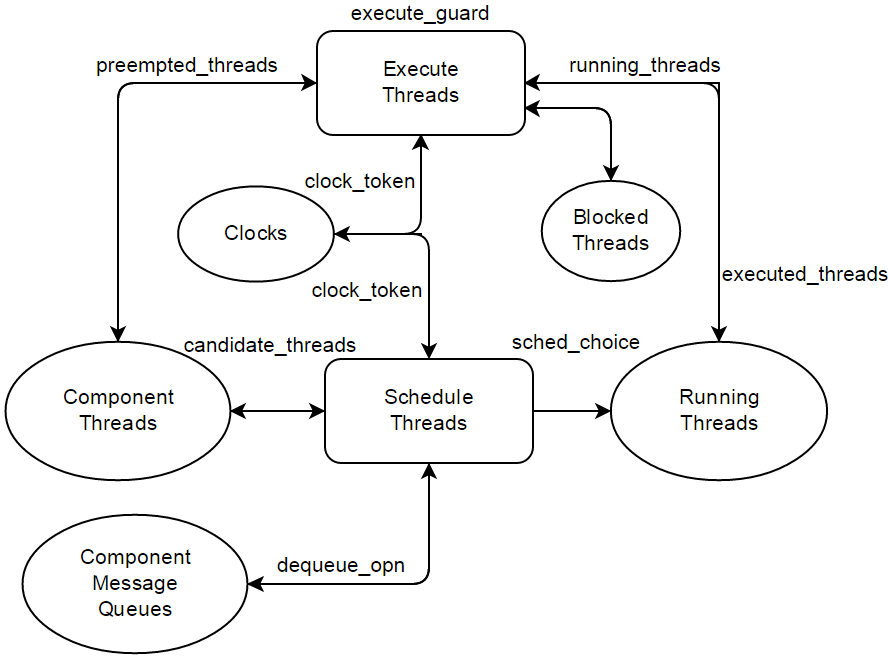
\includegraphics[width=0.40\textwidth]{figs/Thread_Execution.png}
	\caption{Component Thread Execution Cycle}
	\label{fig:Thread_Execution}
\end{figure}

If the highest priority thread is not already servicing an operation request, the highest priority operation from \emph{Component Message Queues} is dequeued and scheduled for execution (held by $O_{CT}$). The scheduled thread is placed in \emph{Running Threads}. %The guard on \emph{Schedule Thread} ensures that the highest priority thread in the currently running partition is scheduled first. 

When a thread token is marked as running, the model checks to see if the thread execution has any effect on itself or on other threads. These state changes are updated using the transition \emph{Execute Thread} which also handles time progression. Keeping track of $Value_{NC}$, the thread is preempted at each clock tick. This loop repeats forever, as long as there are no system-wide deadlocks. 

%It must be noted that system-critical processes such as deployment and fault management processes running periodically (or sporadically) at higher priorities than component processes are not necessarily affected by temporal partitioning. Such processes are scheduled to execute in a \emph{SYSTEM} partition when ever ready. Therefore when simulating the scheduling of such process threads, $TPS_{Node_{NC}}$ in equation \ref{eq:NC} is ignored.




